% !Mode:: "TeX:UTF-8"

\begin{frame}{第二十四讲、曲面积分}
	\linespread{1.5}
	\begin{enumerate}
	  \item {\bf 内容与要求}{\b (\S 12.3)}
	  \begin{itemize}
		\item 理解曲面积分的概念
		\item 熟练掌握曲面积分的计算
		\item 了解曲面积分的应用
	  \vspace{1em}
	  \end{itemize}
	  \item {\bf  课后作业:}
	  \begin{itemize}
	    \item {\b 习题12.3:1,2(1),5,6,9,15(1),18,20}
	  \end{itemize}
	\end{enumerate}
\end{frame}

\section{对面积的曲面积分}

\begin{frame}{求空间曲面的面积}
	\linespread{1.2}
	\begin{exampleblock}{{\bf 例1}\hfill}
		求空间曲面$\Sigma:z=x,(x,y)\in D$的面积,其中:
		\begin{enumerate}
		  \item $D:\,0\leq x\leq 1,\,0\leq y\leq 1$
		  \item $D:\,x^2+y^2\leq 1$
		\end{enumerate}
	\end{exampleblock}\pause 
	\begin{columns}
		\column{.5\textwidth}
			\begin{center}
				\resizebox{!}{3.5cm}{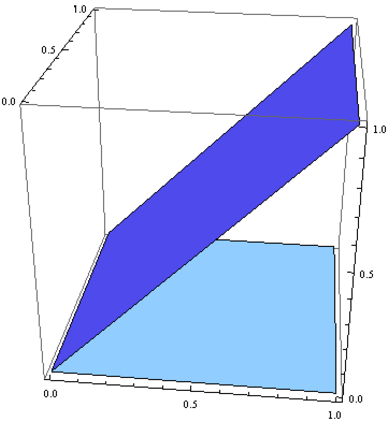
\includegraphics{./images/ch12/ssquare.pdf}}
			\end{center}
		\column{.5\textwidth}\pause 
			\begin{center}
				\resizebox{!}{3.9cm}{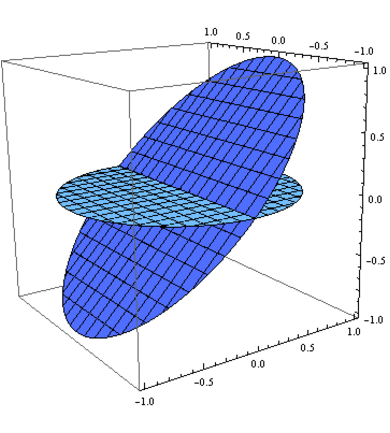
\includegraphics{./images/ch12/scircle.pdf}}
			\end{center}
	\end{columns}
\end{frame}

\begin{frame}{求空间曲面的面积}
	\linespread{1.2}
	{\bf 如何求空间曲面$\Sigma:\,z=f(x,y),\,(x,y)\in D$的面积?\pause }
	$$\alert{S=\iint_{\Sigma}\d S\pause
	=\iint_D\sqrt{1+(f\,'_x)^2+(f\,'_y)^2}\d\sigma}$$\pause 
	\begin{exampleblock}{{\bf 例2}\hfill}
% 		设函数$y=f(x)$在区间$[a,b]$上连续可导、非负,证明其
% 		绕$x$轴旋转所得曲面面积为
% 		$$S=2\pi\dint_a^bf(x)\sqrt{1+(f'_x)^2}dx$$
		推导球表面积公式。
	\end{exampleblock}\pause
	$$\alert{S=4\pi R^2}$$
\end{frame}

% \begin{frame}{求空间曲面的面积}
% 	\linespread{1.2}
% 	{\bf 如何求空间曲面$\Sigma:\,z=f(x,y),\,(x,y)\in D$的面积?\pause }
% 	$$\alert{S=\iint_{\Sigma}\d S\pause
% 	=\iint_D\sqrt{1+(f'_x)^2+(f'_y)^2}\d\sigma}$$\pause 
% 	\begin{exampleblock}{{\bf 例2}\hfill}
% % 		设函数$y=f(x)$在区间$[a,b]$上连续可导、非负,证明其
% % 		绕$x$轴旋转所得曲面面积为
% % 		$$S=2\pi\dint_a^bf(x)\sqrt{1+(f'_x)^2}dx$$
% 		推导球表面积公式。
% 	\end{exampleblock}\pause
% 	$$\alert{S=4\pi R^2}$$
% \end{frame}

\begin{frame}{对面积的曲面积分}
	\linespread{1.2}
	\begin{exampleblock}{{\bf 例3}\hfill}
		设空间曲面$\Sigma:\,z=f(x,y),\,(x,y)\in D$的面密度函数为
		$f(x,y,z)$,求其质量。
	\end{exampleblock}\pause 
	$$\alert{M=\iint_{\Sigma}f(x,y,z)\d S}$$\pause 
	\begin{itemize}
	  \item {\bf 应用:}\pause 质心、\pause 转动惯量、\pause 万有引力\pause 
	  \item {\bf 性质:}\pause 线性性、\pause 曲面的可加性
	\end{itemize}
\end{frame}

\begin{frame}{对面积的曲面积分的计算}
	\linespread{1.2}\pause 
	\begin{exampleblock}{{\bf 例4}\hfill}
		计算曲面积分
		$$I=\oiint_{\Sigma}x^2\d S,$$
		其中$\Sigma$为$x+y+z=1$和坐标平面所围立体的表面。
	\end{exampleblock}\pause 
	\alert{{\bf 步骤:}选择投影方向\pause $\to$写出面积微元\pause $\to$计算二重积分}
\end{frame}

\begin{frame}
	\linespread{1.2}
	\begin{exampleblock}{{\bf 例5}\hfill}
		计算曲面积分
		$$\iint_{\Sigma}z\d S,$$
		其中$\Sigma$为柱面$x^2+y^2=1$夹在平面$z=0$和$z=1+x$之间
		的部分。
	\end{exampleblock}
\end{frame}

\begin{frame}
	\linespread{1.2}
	\begin{exampleblock}{{\bf 例6}\hfill}
		设函数$y=f(x)$在区间$[a,b]$上连续可导、非负,证明其
		绕$x$轴旋转所得曲面面积为
		$$S=2\pi\dint_a^bf(x)\sqrt{1+(f\,'_x)^2}\d x$$
	\end{exampleblock}
\end{frame}

\section{对坐标的曲面积分}

\begin{frame}{流过空间曲面的流量}
	\linespread{1.2}
	\begin{exampleblock}{{\bf 例7}\hfill}
		已知曲面$\Sigma:\,z=f(x,y),\,(x,y)\in D$和流速场
		$$\bm{v}(x,y,z)=(P(x,y,z),Q(x,y,z),R(x,y,z)),$$
		求经过该曲面的流量。
	\end{exampleblock}\pause 
	\alert{{\bf 约定:}沿给定法方向流过$\Sigma$的流量为正,反之为负}
	\invisible{$$\alert{\Phi=\iint_{\Sigma}\bm{v}\cdot\bm{n}dS}$$
	其中$\bm{n}$沿曲面正向的单位法向量。}
\end{frame}

\begin{frame}{空间曲面的方向}
	\linespread{1.2}
	\begin{enumerate}
	  \item {\bf 双侧曲面:}
	  \begin{itemize}
	    \item {\b 封闭曲面:外侧为正,内侧为负}
	    \item 开放曲面:任取一侧为正,一侧为负
	  \end{itemize}
	  \item {\bf 单侧曲面:}无方向
	\end{enumerate}
	\begin{center}
		\resizebox{!}{2.5cm}{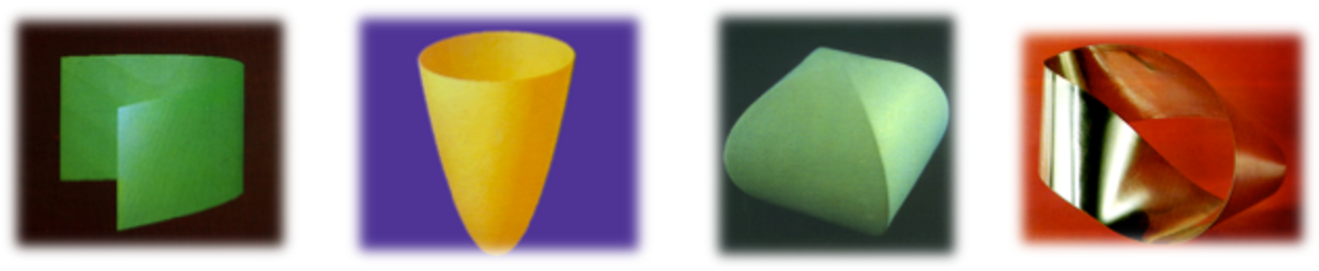
\includegraphics{./images/ch12/ss.pdf}}
	\end{center}
\end{frame}

\begin{frame}{流过空间曲面的流量}
	\linespread{1.2}
	\begin{exampleblock}{{\bf 例8}\hfill}
		已知曲面$\Sigma:\,z=f(x,y),\,(x,y)\in D$和流速场
		$$\bm{v}(x,y,z)=(P(x,y,z),Q(x,y,z),R(x,y,z)),$$
		求经过该曲面的流量。
	\end{exampleblock}
	\alert{{\bf 约定:}沿给定法方向流过$\Sigma$的流量为正,反之为负}\pause
	$$\alert{\Phi=\iint_{\Sigma}\bm{v}\cdot\bm{n}\d S}$$
	\pause 其中$\bm{n}$沿曲面正向的单位法向量。
\end{frame}

\begin{frame}{对坐标的曲面积分}
	\linespread{1.2}
	$$\alert{\Phi=\iint_{\Sigma}\bm{v}\cdot\bm{n}\d S}$$
	\pause 注意到
	$$\bm{n}\d S=(\d\sigma_{yz},\d\sigma_{zx},\d\sigma_{xy})
	=(\d y\d z,\d z\d x,\d x\d y),$$
	\pause 故
	$$\alert{\Phi=\iint_{\Sigma}P(x,y,z)\d y\d z
	+Q(x,y,z)\d z\d x+R(x,y,z)\d x\d y}$$
\end{frame}

\begin{frame}{对坐标的曲面积分的计算}
	\linespread{1.2}
	\begin{exampleblock}{{\bf 例9}\hfill}
		已知曲面$\Sigma:\,z=f(x,y),\,(x,y)\in D$,计算
		$$I=\iint_{\Sigma}R(x,y,z)\d x\d y$$
	\end{exampleblock}\pause 
	\begin{enumerate}
	  \item {\bf 曲面的参数方程:}\pause $x=x,y=y,z=z(x,y)$\pause 
	  \item {\bf 判断曲面方向:}若曲面正向与$z$轴成锐角,取正号;反之为负\pause 
	\end{enumerate}
	$$\alert{I=\pm\iint_DR(x,y,z(x,y))\d x\d y}$$
\end{frame}

\begin{frame}
	\linespread{1.2}
	\begin{exampleblock}{{\bf 例10}\hfill}
		计算曲面积分
		$$I=\oiint_{\Sigma}xyz\d x\d y,$$
		其中$\Sigma$由四分之一单位球面($x\geq 0,y\geq 0$)和
		$x=0$,
		
		$y=0$共同组成。
	\end{exampleblock}
\end{frame}

\section{曲面积分的应用}

\begin{frame}{曲面积分的应用}
	\linespread{1.5}\pause 
	\begin{enumerate}
	  \item {\bf 对面积的曲面积分:}\pause 
	  \begin{itemize}
	    \item 曲面的质量\pause 
	    \item 质心\pause 
	    \item 转动惯量\pause 
	    \item 万有引力\pause 
	  \end{itemize}
	  \item {\bf 对坐标的曲面积分:}\pause 
	  \begin{itemize}
	    \item 流量
	  \end{itemize}
	\end{enumerate}
\end{frame}

\begin{frame}{曲面积分的应用}
	\linespread{1.2}
	\begin{exampleblock}{{\bf 例11}\hfill}
		设半球壳$z=\sqrt{R^2-x^2-y^2}$的密度为常数$\mu$,求:
		\begin{enumerate}
		  \item 半球壳的质心;
		  \item 半球壳关于$z$轴的转动惯量。
		\end{enumerate}
	\end{exampleblock}
	\bigskip\pause 
	\begin{exampleblock}{{\bf 例12}\hfill}
		将半径为$R$的球体置于水中,顶部与水面相切,求球的上半部分所受水的压力。
	\end{exampleblock}
\end{frame}

\begin{frame}{曲面积分的应用}
	\linespread{1.2}
	\begin{exampleblock}{{\bf 例13}\hfill}
		已知流速场$\bm{v}=(0,yz,z^2)$,求穿过柱面
		$y^2+z^2=1 $
		
		$(z\geq 0)$被$x=0$和$x=1$所夹部分的流量,
		取曲面上侧为其正向。
	\end{exampleblock}
\end{frame}

\begin{frame}{小结}
	\linespread{1.2}
	\begin{enumerate}
	  \item 对面积的曲面积分
	  $$S=\iint_{\Sigma}\d S=\iint_D\sqrt{1+(f\,'_x)^2+(f\,'_y)^2}\d\sigma_{xy}$$
	  \item 对坐标的曲面积分
	  \begin{itemize}
	    \item 曲面的方向性
	  \end{itemize}
	  \item 曲面积分的应用
	\end{enumerate}
	\hrule
	\begin{center}
		\ba{注意和曲线积分的概念与方法进行类比}
	\end{center}
\end{frame}

%=====================================

% \begin{frame}{title}
% 	\linespread{1.2}
% 	\begin{exampleblock}{{\bf title}\hfill}
% 		123
% 	\end{exampleblock}
% \end{frame}
% 
% \begin{frame}{title}
% 	\linespread{1.2}
% 	\begin{block}{{\bf title}\hfill}
% 		123
% 	\end{block}
% \end{frame}